\documentclass[tikz,border=10pt]{standalone}
\usepackage{pgfplots}
\pgfplotsset{compat=1.18}
\usepackage{amsmath}
\usepackage{amssymb}
\definecolor{mantis}{RGB}{0, 105, 62}
\begin{document}
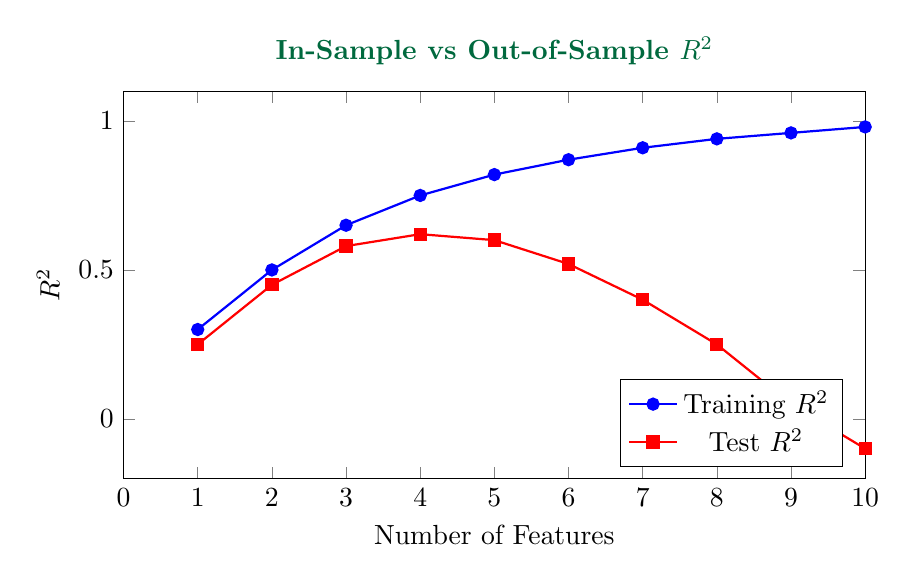
\begin{tikzpicture}
\begin{axis}[
    width=11cm,
    height=6.5cm,
    xlabel={Number of Features},
    ylabel={$R^2$},
    xmin=0, xmax=10,
    ymin=-0.2, ymax=1.1,
    legend pos=south east,
    title={\textbf{In-Sample vs Out-of-Sample $R^2$}},
    title style={font=\bfseries\color{mantis}},
]
% Training R^2 (always increasing)
\addplot[domain=1:10, samples=10, color=blue, thick, mark=*] coordinates {
    (1, 0.3) (2, 0.5) (3, 0.65) (4, 0.75) (5, 0.82) (6, 0.87) (7, 0.91) (8, 0.94) (9, 0.96) (10, 0.98)
};
% Test R^2 (increases then decreases)
\addplot[domain=1:10, samples=10, color=red, thick, mark=square*] coordinates {
    (1, 0.25) (2, 0.45) (3, 0.58) (4, 0.62) (5, 0.60) (6, 0.52) (7, 0.40) (8, 0.25) (9, 0.05) (10, -0.1)
};
\legend{Training $R^2$, Test $R^2$}
\end{axis}
\end{tikzpicture}
\end{document}
